%!TEX root = ../notas_de_clase.tex

\section{Aprendizaje no supervisado}

\subsection{Reducción de dimensionalidad}

El problema de reducción de dimensionalidad consiste con construir una representación de dimensión estrictamente menor que los datos originales con la finalidad de interpretar de mejor forma la información contenida en nuestros datos así como también disminuir el costo computacional en el entrenamiento.

\subsubsection{Análisis de componentes principales (PCA)}

Consideremos ahora un conjunto de observaciones de $\{\x_i\}_{i=1}^N\subset\R^M$, donde denotamos $\x_i=[x_{i1},x_{i2},\ldots,x_{iM}]^\top$. Podemos entender que el elemento $x_{ij}$ corresponde al valor del atributo $j$ para la observación $i$. 

Notemos que cada observación puede descomponerse en la base canónica $\{\e_i\}_{i=1}^M$ de $\R^M$ de la forma 
\begin{equation}
	\x_i = x_{i1}\e_1 +  x_{i2}\e_2 + \cdots + x_{iM}\e_M 		
\end{equation}
Notemos que es posible representar cada vector $\x_i$ mediante una cantidad $M'<M$ de términos, truncando la representación anterior, es decir,  
\begin{equation}
	\x_i \approx \sum_{j=1}^{M'} x_{i\sigma(j)}\e_{\sigma(j)}
\end{equation}
donde $\sigma:\{1,2,\ldots,M\}\mapsto\{1,2,\ldots,M\}$ es una permutación que prioriza las coordenadas más representativas de los datos. Dichas aproximaciones de las observaciones $\{\x_i\}_{i=1}^N$ son una versión de baja dimensión, entonces, naturalmente nos podemos hacer la siguiente pregunta: dada una dimensión $M'<M$  ¿es efectivamente un subconjunto de los vectores canónicos la mejor base para descomponer las observaciones?  ¿cómo encontramos la \emph{mejor} base?

\begin{figure}[H]
	\centering
	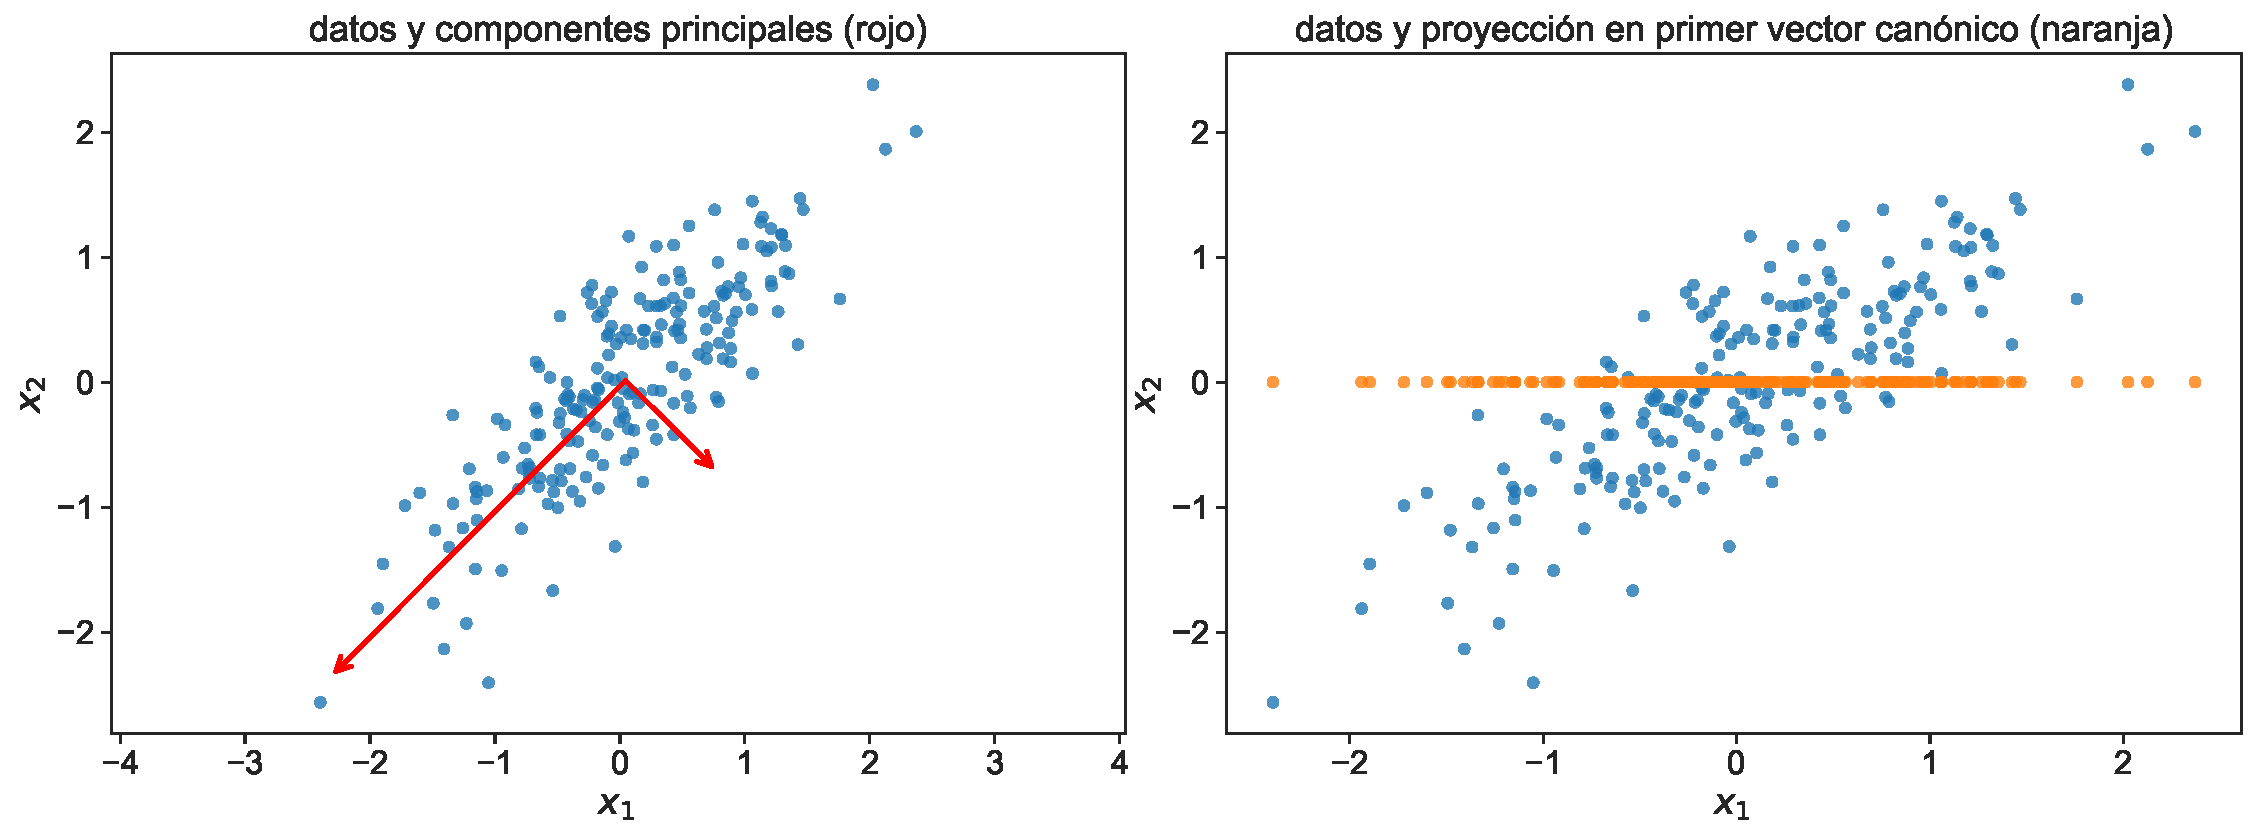
\includegraphics[width=0.6\textwidth]{img/cap6_pca.pdf}
	\caption{Base ortogonal de $\R^2$ formada por las componentes principales de los datos. Se observa en este caso que ninguna de las componentes principales corresponde a un vector de la base canónica. El eje que cruza los cuadrantes 1 y 3 corresponde a $\cvector_1$ y el otro, a $\cvector_2$.}
	\label{fig:ej_fda_1}
\end{figure}

La respuesta a la primera pregunta es, en la mayoría de los casos, negativa. Esto es porque los elementos de la base canónica, por sí solos, conllevan poca información estructural que puede ser encontrada en los vectores observados. En particular, consideremos el caso en donde solo se dispone de dos observaciones $\{\x_1, \x_2\}$, si $M'=2$, entonces una descomposición que garantiza error nulo es simplemente elegir $\x_1$ y $\x_2$ como bases de la nueva descomposición, donde los coeficientes estarían dados por $[1,\ 0]^\top$ y $[0,\ 1]^\top$.\\

Para encontrar la \emph{mejor} base, lo primero que se requiere es definir qué se entiende por \emph{mejor}. Nos enfocaremos en determinar una base cuyos componentes \textbf{ordenados} $\cvector_1,\cvector_2,\ldots$ capturan las $M'$ direcciones ortogonales de máxima variabilidad de nuestros datos. De esta forma, dado que $\langle\cvector,\x\rangle$ representa la proyección ortogonal de $\x$ sobre $\cvector$, el primer elemento de la nueva base estará dado por 
\begin{equation}
	\cvector_1 = \argmax_{||\cvector||=1} {\langle\cvector,\x\rangle} \label{eq:PCA_max}
\end{equation}
Este criterio es conocido como \textbf{análisis de componentes principales (PCA)}. Notemos que la restricción $||\cvector_1||=1$ es necesaria ya que $\langle\lambda\cvector_1,\x\rangle = \lambda\langle\cvector_1,\x\rangle$ por lo que $\langle\cvector_1,\x\rangle$ puede crecer indefinidamente si no se fija una restricción sobre la norma de $\cvector$. Por esta razón, s.p.g. podemos fijar la norma de $\cvector_1$ en 1 y buscar una base ortonormal. Además, es importante estandarizar los datos:

\begin{itemize}
	\item Características de media nula: la matriz $X$ con $(X)_{ij} = (\x_i)_j$ debe tener columnas con media $0$. Esto se consigue restando la media de la columna a cada una de las entradas de dicha columna. El objetivo de este ajuste es poder centrar los datos.
	\item Varianzas marginales unitarias: si una dimensión tiene una varianza marginal mayor que el resto, esta será más importante en la determinación de la dirección de máxima varianza solo por su magnitud y no por la relación entre variables. La normalización se consigue dividiendo cada entrada de la columna por la desviación estándar de la columna.
\end{itemize}

Como en general no contamos con la distribución de las observaciones $p(\x)$, podemos considerar una aproximación muestral de la varianza en la ecuación \eqref{eq:PCA_max} y resolver 
\begin{align}
	\cvector_1 = \argmax_{||\cvector||=1} \sum_{i=1}^N \langle\cvector,\x_i\rangle^2.\label{eq:PCA_max2}
\end{align}

Podemos ahora usar la siguiente notación
$$
X=\begin{bmatrix}
        \x_1^\top\\
        \vdots\\
        \x_N^\top\\
        \end{bmatrix}=
        \begin{bmatrix}
        {x}_{11}    & \dots & {x}_{1M}  \\
        \vdots          & \ddots& \vdots        \\
        {x}_{N1}    & \dots & {x}_{NM}
        \end{bmatrix}
$$
y reescribir la ecuación \eqref{eq:PCA_max2} como 
\begin{equation}
	\cvector_1 = \argmax_{||\cvector||=1} ||X\cvector||^2 
			= \argmax_{||\cvector||=1} \cvector^\top X^\top X \cvector
			= \argmax_{\cvector} \frac{\cvector^\top X^\top X \cvector}{\cvector^\top \cvector}
			\label{eq:PCA_max3}
\end{equation}

Por otra parte, se tiene la siguiente propiedad:

\begin{lemma}[minimización del cociente de Rayleigh]

Sea $M\in\mathcal{M}_{nn}(\R)$ matriz cuadrada simétrica, entonces, para el cociente de Rayleigh

\begin{equation}
	R(M,x):=\frac{x^\top Mx}{x^\top x}
\end{equation}

Su valor mínimo corresponde al menor valor propio de $M$, y es alcanzado en su vector propio asociado.

\end{lemma}

\begin{proof}
	Dado que $R(M,cx)=R(M,x)$ para todo $c\neq 0$, basta verlo para $\norm{x}=1$, por lo que se puede considerar como una restricción adicional. Por teorema de Lagrange:
	
	\begin{equation}
		L(x,\lambda) = x^\top Mx - \lambda(\norm{x} - 1)\implies \frac{\partial L}{\partial x} = 2x^\top M - 2\lambda x^\top = 0 \implies Mx=\lambda x
	\end{equation}
	
	Por lo tanto, los puntos críticos de lagrangiano son los vectores propios $v_i$ de $M$. Por otra parte:
	
	\begin{equation}
		R(M,v_i)=\frac{v_i^\top Mv_i}{v_i^\top v_i} = \frac{v_i^\top \lambda_i v_i}{v_i^\top v_i} = \lambda_i\in\R \text{ ya que $M$ es simétrica.}
	\end{equation}
	
Por lo tanto, el valor mínimo de $R(M,x)$ es $\lambda_{min}$ y es alcanzado en el vector propio asociado $v_{min}$. Por el mismo argumento, el valor máximo es $\lambda_{max}$ y es alcanzado en $v_{max}$.
\end{proof}

De esta forma, dado que $X^\top X$ es simétrica, su cociente de Rayleigh es maximizado en el vector propio asociado al valor propio máximo de $X^\top X$. Consecuentemente, la proyección de una observación $\x_i$ en la dirección de máxima varianza, o bien la \emph{primera componente principal}, está dada por 
\begin{equation}
	\x_i^{(1)} = \langle \x_i, \cvector_1 \rangle
\end{equation}
donde $\cvector_1$ es el vector propio asociado al mayor valor propio de la matriz de covarianza muestral $XX^\top$.\\

El cálculo de las siguientes componentes se realiza de forma iterativa sobre los residuos del conjunto de observaciones con respecto a las componentes anteriores. De esta forma, PCA encuentra una nueva base ortonormal tal que las componentes maximicen la variabilidad donde en algunos casos se puede perder intepretabilidad de las nuevas características generadas, pues son combinaciones lineales de las características originales de los datos. A pesar de esto, utilizando las primeras 2 o 3 componentes PCA se pueden visualizar datos de alta dimensionabilidad de forma ilustrativa.


\subsubsection{Kernel PCA}
El método Kernel PCA es similar a PCA, pero esta vez se utiliza el truco del kernel para proyectar los datos. En ese sentido, en vez de calcular la matriz de covarianza empírica $X^\top X$, se utiliza la matriz de Gram dada por un kernel $K$ donde

$$
K_{ij} = K(x_i,x_j) = \langle\phi(x_i),\phi(x_j)\rangle
$$

Luego, se realiza PCA utilizando dicha matriz.\\

En la Figura \ref{fig:kpca} se puede observar un ejemplo en que el resultado de linear PCA no es suficiente, puesto que el problema es simétrico, mientras que KPCA realiza una correcta separación de ambos clusters.

\begin{figure}[ht]
    \centering
    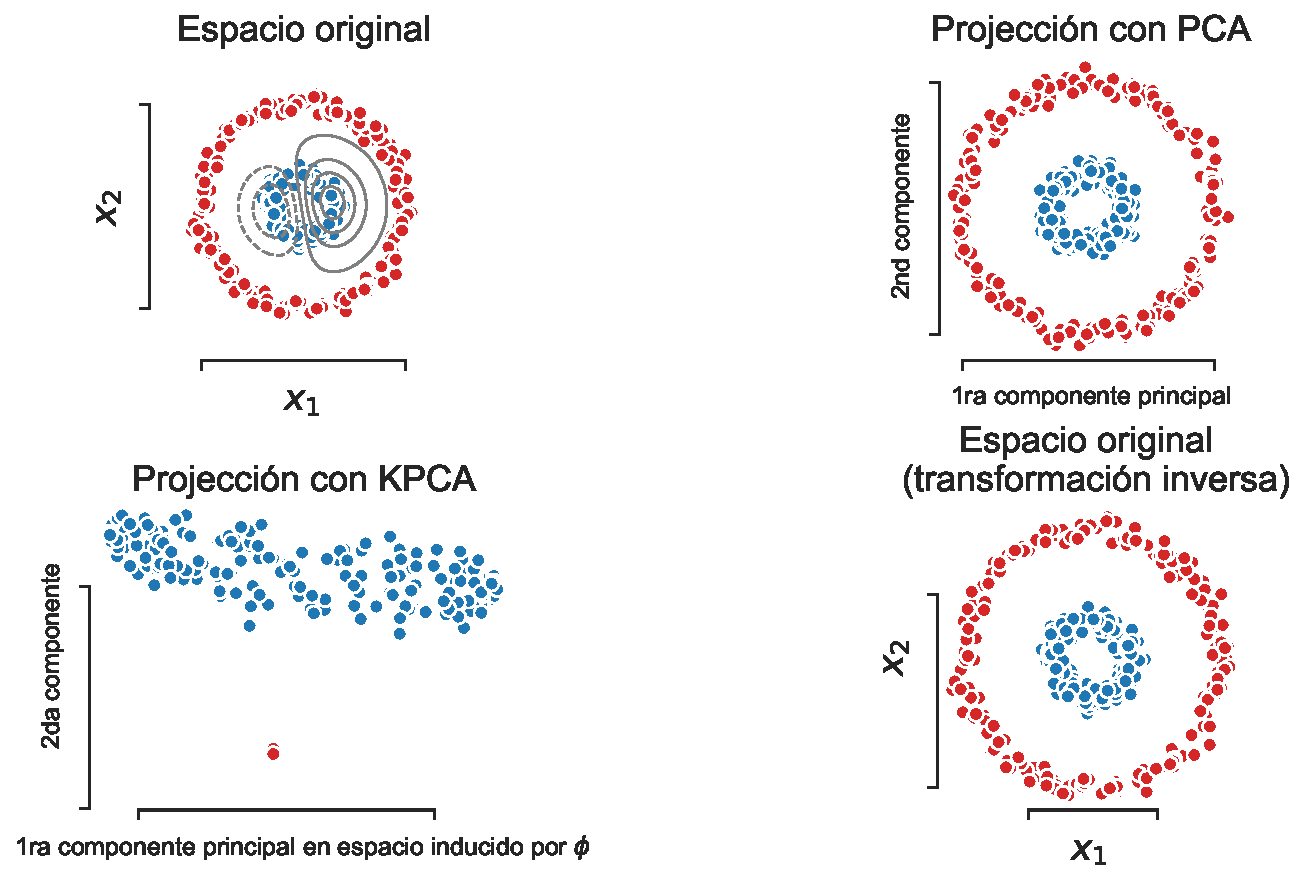
\includegraphics[width=0.7\linewidth]{img/cap6_kpca.pdf}
    \caption{Ejemplo de KPCA sobre un conjunto de datos que no es linealmente separable.}
    \label{fig:kpca}
\end{figure}

\subsubsection{Probabilistic PCA}
PCA probabilístico (PPCA) tiene su inspiración en que PCA se puede expresar como la solución vía máxima verosimilitud de un modelo probabilístico de variable latente. De este modo, PPCA propone un método iterativo para obtener la solución evaluando solo cierto número de componentes, sin necesidad de calcular la matriz de covarianza empírica.

El modelo probabilístico para PCA en el que se inspira PPCA es el siguiente:\\

Sean $(x_i)_{i=1}^N\subset \mathbb{R}^M$ los elementos observados, inputs o variables y $z\in \mathbb{R}^l$ una variable latente explícita correspondiente al espacio de las componentes principales. Bajo la hipótesis de un modelo de observación lineal:

\begin{equation}
	x=Wz+\mu+\epsilon
\end{equation}

Donde $\epsilon\sim\mathcal{N}(0,\sigma^2)$ es un sumando de ruido y $W\in \R^{M\times l}$, $\mu \in \R^M$ y $\sigma^2$ son parámetros a determinar, se define el siguiente prior para $z$:

\begin{equation}
p(z) = \mathcal{N}(0,\eye)
\end{equation}

De este modo, la distribución condicional de x dado z también es gaussiana:

\begin{equation}
p(x|z) = \mathcal{N}(Wz+\mu,\sigma^2\eye)
\end{equation}

Notemos que no se pierde generalidad tomar el prior para $z$ con media cero y varianza unitaria, puesto que si se toma otro prior más general, se produce el mismo modelo.\\


Dado que tenemos un modelo paramétrico probabilístico, podemos estimar los parámetros con máxima verosimilitud. Dado los datos $\mathcal{D} = \{x_i\}_{i=1}^N$, la log-verosimilitud está dada por:

\begin{align}
\log p(\mathcal{D}|W,\mu, \sigma^2) & = \sum_{i=1}^N \log p(x_i|W,\mu, \sigma^2)\\
& = \frac{NM}{2}\log (2\pi) - \frac{N}{2}log|C| - \frac{1}{2}\sum_{i=1}^N (x_i-\mu)^T C^{-1} (x_i-\mu),
\end{align}

con $C = WW^T + \sigma^2 I$.

Usando la condición de primer orden obtenemos

\begin{equation}
	\mu = \bar{x} = \frac{1}{N}\sum_{i=1}^N x_i
\end{equation}

De esta manera tenemos la función de log-verosimilitud completa:

\begin{align}
    \log p(X, Z|W, \mu, \sigma^2) = \sum_{i=1}^N \{\log p(x_i|z_i) + \log p(z_i)\}
\end{align}

y evaluando en $\mu = \bar{x}$

\begin{align}
\notag \mathbb{E}[ p(X,Z |W, \mu, \sigma^2) ] =  -\sum_{i=1}^N \Bigg\{ &\frac{l}{2} \log (2\pi \sigma^2)\\
\notag & + \frac{1}{2}\text{Tr}(\mathbb{E}[z_iz_i^T])\\
\notag & \frac{1}{2\sigma^2}||x_i - \mu||^2 - \frac{1}{\sigma^2}\mathbb{E}[z_i]^T W^T (x_i - \mu)\\
& \frac{1}{2\sigma^2} \text{Tr}(\mathbb{E}[z_iz_i^T]W^T W) \Bigg\}
\end{align}

\subsubsection{Discriminante lineal de Fisher}

Para evitar los artefactos (sesgos) introducidos por clases  asimétricas en el uso de mínimos cuadrados para clasificación, es posible interpretar el problema de clasificación como uno de \emph{reducción de dimensionalidad}, en donde la reducción consiste representar nuestros datos  en solo una dimensión, la cual representa su (grado de pertenencia a una) clase. Con este objetivo en mente, consideremos el problema de clasificación binaria de $x\in \R^M$, donde proyectamos $x$ en un espacio \textbf{unidimensional} con respecto a un vector $a\in\R^M$ de acuerdo a:

\begin{equation}
	y = a^\top x,
\end{equation}

donde podemos definir un umbral $b$ para asignar $x$ a $\cC_1$ si $y+b\geq 0$ y $x$ a $\cC_2$ en caso contrario. Notemos que de esta forma recuperamos el modelo lineal para clasificación.\\

En general, al proyectar un objeto $M$-dimensional en un espacio  1-dimensional, se pierde gran parte de la información, lo cual genera el hecho de que clases claramente separadas en el espacio $M$-dimensional puedan traslaparse al ser proyectadas a 1 dimensión cuando la elección del vector $a\in\R^M$ no es la mejor. Sin embargo, es posible ajustar el vector $a$ con la finalidad de obtener una proyección de $x$ que maximice el grado de separación entre clases.\\

Con el objetivo de encontrar el vector $a$ que cumple con este requerimiento en base a un conjunto de datos  $\datos$, primero definamos las cardinalidades de clases mediante $N_1 = |\{x\in\datos:x\in\cC_1\}|$ y $N_2 = |\{x\in\datos:x\in\cC_2\}|$, lo cual permite calcular los promedios muestrales (centros de masa) de cada  clase mediante: 
\begin{equation}
	\mu_1=\frac{1}{N_1}\sum_{n\in\mathcal{C}_1}x_n
	\quad\quad\quad
	\mu_2=\frac{1}{N_2}\sum_{n\in\mathcal{C}_2}x_n
\end{equation}
La medida más simple de separación entre las proyecciones de las clases sobre $a$ es la distancia entre las medias  de sus proyecciones:
\begin{equation}
	m_1 - m_2 = a^\top(\mu_1-\mu_2)
\end{equation}
donde $m_k= a^\top\mu_k$ corresponde al promedio de los elementos de  la clase $\mathcal{C}_k$ proyectado sobre el  vector $a$ (centro de masa sobre la recta). Consecuentemente, el vector $a$ que maximiza la distancia entre la proyección de clases es el que maximiza la expresión anterior. Sin embargo, esta expresión puede ser arbitrariamente grande si escalamos $a$, por lo que se fijará $\left \| a \right \|_2=1$. Además, por la desigualdad de Cauchy-Schwarz, $|a^\top(\mu_1-\mu_2)|\leq \norm{a}\norm{\mu_1-\mu_2}$ con igualdad si y solo si los vectores son paralelos. De este modo, se llega a que $a\propto(\mu_1-\mu_2)$. \\

Una desventaja de este enfoque, en el cual se ha ignorado la dispersión de las clases y solo se ha considerado su media, es que pueden existir 2 clases bien separadas en el espacio $M$-dimensional, pero que al proyectar los datos sobre la recta que une sus promedios, las proyecciones de cada clase se traslapen. 

\begin{figure}[H]
	\centering
	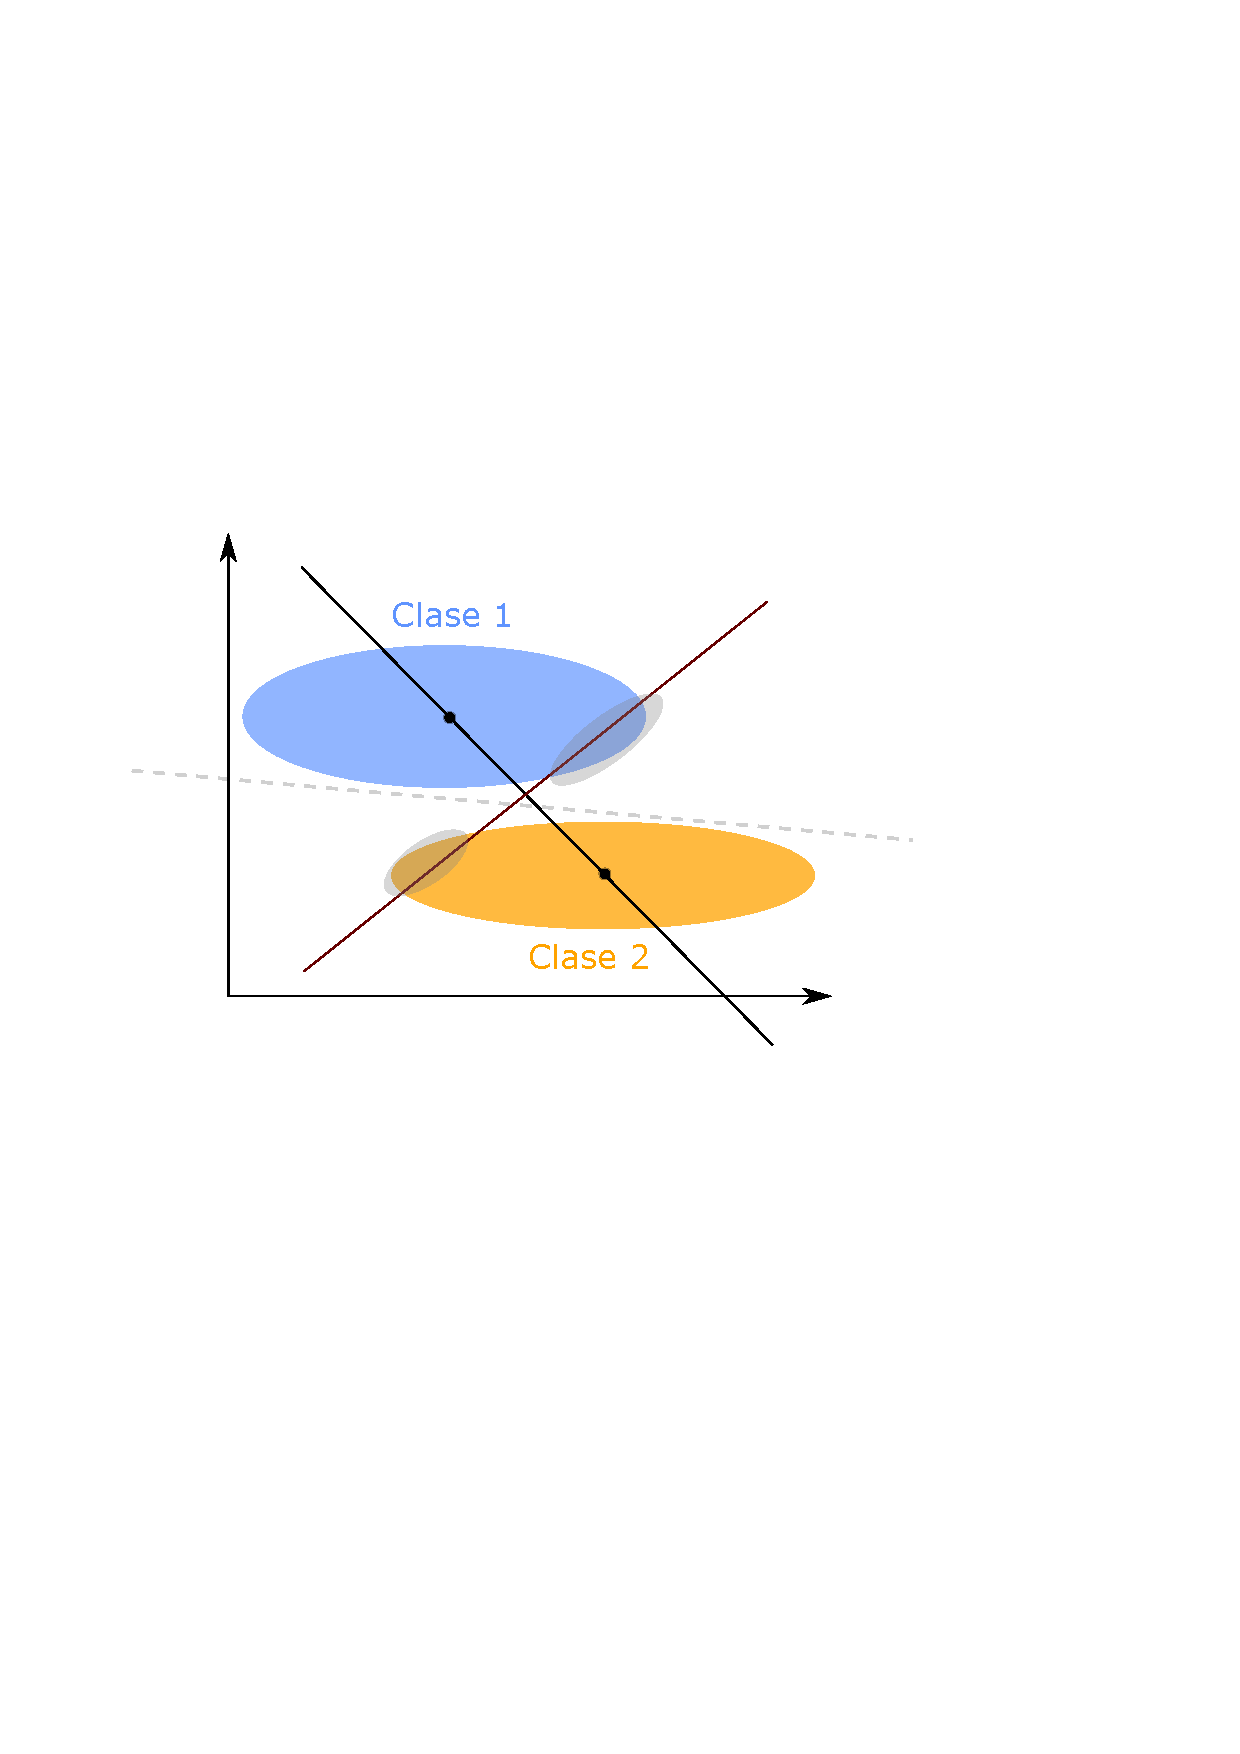
\includegraphics[width=0.6\textwidth]{img/cap6_fisher.pdf}
	\caption{Superposición de las proyecciones al considerar únicamente la recta que une las medias de clase. La recta roja determina la región de decisión y la recta segmentada muestra un posible hiperplano separador.}
	\label{fig:ej_fda_2}
\end{figure}

Para resolver este problema, Fisher propuso maximizar no solo distancia entre las (medias de las) clases proyectadas, sino que adicionalmente minimizar la dispersión de los elementos de una misma clase, con el objetivo de disminuir el traslape entre las proyecciones de las clases. Como medida de dispersión, definimos la varianza muestral proyectada de los elementos de la clase $\cC_k$ mediante
\begin{align}
	s_k^2 &= \sum_{n\in \mathcal{C}_k}(a^\top(x_n-\mu_k))^2\\
	&= \sum_{n\in \mathcal{C}_k}(y_n-m_k)^2,
\end{align}
Donde el factor de correción $\frac{1}{N_k-1}$ fue omitido ya que de lo contrario, todas las clases pesarían lo mismo sin importar la cantidad de elementos de la clase. Lo anterior nos permite definir la siguiente función objetivo
\begin{equation}
J(a) = \frac{m_1-m_2}{s_1^2+s_2 ^2},
\end{equation}
donde explícitamente vemos la discrepancia ``inter'' clases en el numerador y la discrepancia  ``intra '' clases en el denominador. Adicionalmente, podemos expresar este costo directamente como función del vector de proyección $a$:
\begin{equation}
	J(a) = \frac{a^\top S_B a}{a^\top S_Wa},
\end{equation}
donde la matriz de covarianza entre clases $S_B$ y matriz total de covarianza dentro de clases $S_W$ están respectivamente dadas por
\begin{align}
	S_B &= (\mu_1-\mu_2)(\mu_1-\mu_2)^\top\\
	S_W &= \sum_{n\in \cC_1}(x_n-\mu_1)(x_n-\mu_1)^\top +
	\sum_{n\in \cC_2}(x_n-\mu_2)(x_n-\mu_2)^\top. 
\end{align}
Aplicando la condición de primer orden para $J(a)$, obtenemos que el vector $a$ óptimo debe cumplir
\begin{equation}
	(a^\top S_B a)S_W a = (a^\top S_W a)S_B a.	
\end{equation}
Sin embargo, notemos que la norma del vector  $a$ es irrelevante, solo interesa su orientación, con lo que  ignorando los escalares $(a^\top S_B a)$ y $(a^\top S_W a)$ tenemos que la relación de optimalidad es $S_W a \propto S_B a$. Además, por la definición de $S_B$, sabemos que $S_B a\propto(\mu_1-\mu_2)$, con lo que la relación de optimalidad se convierte en es $S_W a \propto (\mu_1-\mu_2)$. Consecuentemente, el vector optimo $a$ en el  criterio de Fisher debe cumplir
\begin{equation}
	a \propto S_W^{-1}(\mu_1-\mu_2).
\end{equation}

La Figura \ref{fig:ej_fda_1} muestra el  discriminador lineal que solo considera los promedios a la  izquierda y la corrección de Fisher a la derecha. Observemos cómo el incluir una medida de la dispersión de los datos es clave para lograr un mejor discriminador.

\begin{figure}[H]
	\centering
	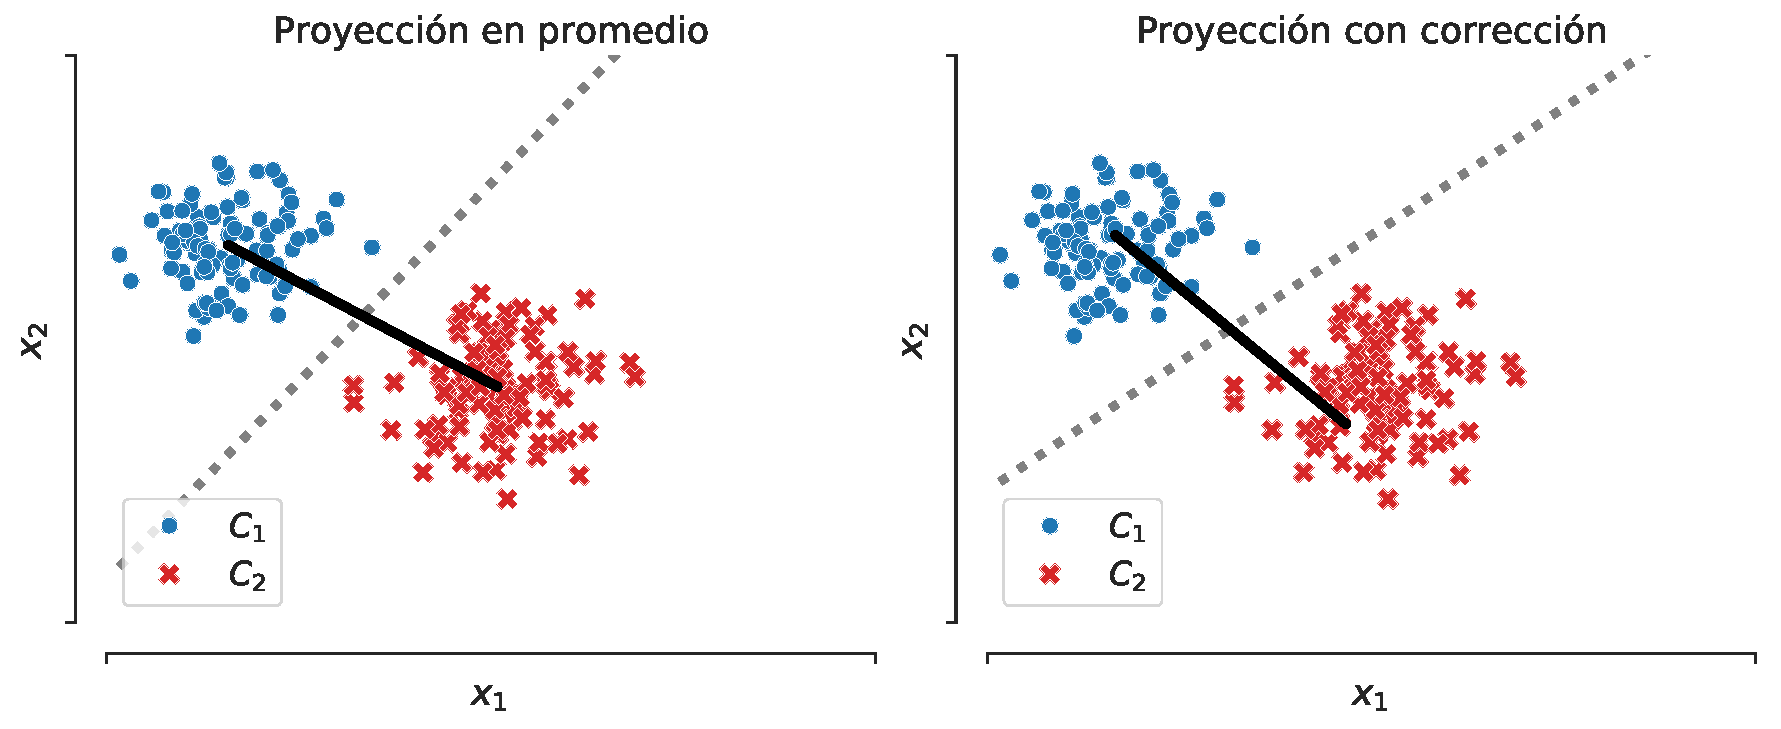
\includegraphics[width=0.8\textwidth]{img/cap6_dos_clases_proyeccion.pdf}
	\caption{Discriminador lineal considerando solo la media entre clases (izquierda) y  su extensión mediante la corrección de Fisher que incorpora la varianza muestral de los datos.}
	\label{fig:ej_fda_3}
\end{figure}

\subsubsection{Compressed Sensing }

\textit{Compressed Sensing} es una técnica de reducción de dimensionalidad basada en la hipótesis previa de que el vector original de los datos es \textit{sparse} en alguna base. \\

Como motivación, sea $x \in \R^d$ con a lo más $s$ coordenadas distintas de $0$. Es decir: 
$$
\| x \|_0 = | \left \{i: x_i \not = 0 \right \} \leq s.
$$

En esta situación, $x$ puede ser comprimido si es representado por $s$ pares de la forma \textit{(índice, valor)}. Además, esta compresión no tiene pérdidas sobre la información de $x$, pues este vector se puede reconstruir exactamente en base a estos pares.\\ 

Ahora, dada $U$ una matriz ortonormal fija, supongamos que $x = U \alpha$, con $\alpha$ un vector sparse, i.e $\| \alpha \|_0 \leq s$. Entonces, estamos suponiendo que existe otra base de $\R^d$ bajo la cual $x$ es un vector \textit{sparse}. Si bien esta suposición puede parecer ingenua en un inicio, muchos vectores resultan cumplir esta propiedad. Ahora, en este caso ¿Es posible comprimir $x$ usando sólo $s$ pares como los mencionados anteriormente? \\

Una forma simple de hacer lo anterior es multiplicar $x$ por $U^{T}$, y luego representar el vector resultante $\alpha $ por los pares deseados. Sin embargo, este proceso requiere primero guardar $x$, y luego multiplicar por $U^{T}$, lo que naturalmente levanta la pregunta de si es realmente necesario guardar una gran cantidad de información que luego será desechada. ¿Será posible medir lo que no será desechado y trabajar con esta parte de $x$ directamente?\\

La respuesta es si, y está basada en un resultado clave: Una transformación lineal $x$ puede comprimir $x$ sin pérdida de información. Para profundizar esto, se requiere la siguiente definición: 

\begin{definition}
Una matriz $U \in \R^{n \times d}$ es $(\epsilon,s)$- RIP (\textit{Restricted Isoperimetric Property}) si para todo $x \not =0$, tal que $\|x\|_0 \leq s$, se cumple: 
$$
\left |\dfrac{\| Ux\|^{2}_2}{\|x\|_2^{2}} - 1 \right | \leq \epsilon 
$$
\end{definition}

Teniendo en cuenta lo anterior, el siguiente Teorema es la razón por la cuál esta técnica tiene sentido.

\begin{theorem}
Sea $\epsilon <1$ y $U \in \R^{n \times d}$ una matriz $(\epsilon, 2s)$-RIP. Sea $x \not = 0$ un vector en $\R^d$ tal que $\| x \|_0 \leq s$, e $y = Ux$ la compresión de $x$. Entonces el vector reconstruído: 
$$
\bar{x} \in \underset{v: Wv = y}{\argmin}
$$
cumple $\bar{x} = x$. 
\end{theorem}

Luego, basándonos el Teorema anterior, es posible comprimir $x$ sin pérdida alguna, siempre y cuando logremos encontrar la matriz $U$ adecuada. 


\subsubsection{PCA vs. Compressed Sensing}

Teniendo en cuenta los dos métodos de reducción de dimensionalidad aquí mencionados, es natural preguntarse cuál de ellos se debe usar en diferentes situaciones.  \\

En primer lugar, es importante recordar que si se cumplen las suposiciones de cada técnica, es posible reconstruir perfectamente la información de dimensión reducida. \\

La pregunta clave es qué es lo que se quiere comprimir. Si son vectores que cumplen con tener una gran cantidadad de $0$, compressed sensing será probablemente una ejor opción que PCA. Un ejemplo podría ser trabajar con vectores canónicos en $\R^d$. Por otra parte, si no se tiene mucha información con respecto a lo que se quiere comprimir, es mejor ocupar PCA pues es un método más efectivo cuando los datos tienen ruido. Por otra parte, si tenemos $N$ datos que están exactamente en un subespacio de dimensión $n$ (por ejemplo un hiperplano), PCA es la alternativa recomendada pues nada asegura que se cumplan las condiciones para hacer comressed sensing. 


\subsubsection{Otros métodos de reducción de dimensionalidad}

\begin{itemize}
    \item \textbf{Escalamiento Multidimensional}
    
    Se busca reducir la dimensión intentando preservar la distancia entre las instancias. \\
    
    En términos prácticos, se comienza con  $x_1, ..., x_n \in \R^{N}$, y $d_{ij}$ la distancia entre $x_i$ y $x_j$. Frecuentemente esta distancia es la distancia euclidiana, sin embargo se pueden elegir también medidas de disimilitud entre los inputs. \\
    
    El escalamiento multidimensional busca encontrar $z_1, ... z_k \in \R^p$ que minimicen la función de stress: 
    $$
    S_M(z_1,...z_k) = \sum_{i \not = j} (d_{ij} - \|z_i - z_j\|)^2.
    $$
    Este escalamiento se conoce como de mínimos cuadrados o de Kruskal–Shephard. Es importante notar que la forma de la función de stress sugiere que un algoritmo de descenso de gradiente es una buena herramienta para minimizarla.
    
    \item \textbf{t-Distributed Stochastic Neighbor Embedding (t-SNE)}
    
    Se busca reducir la dimensionalidad buscando dejar instancias similares cerca y distancias disimilares lejos. Se suele ocupar para visualización, sobre todo para visualizar clusters en data de altas dimensiones. \\
    
    Este método consta, a grandes rasgos, de dos pasos: 
    \begin{enumerate}
        \item En primer lugar, se genera una distribución sobre parejas de inputs, de forma tal que parejas de puntos que se encuentren cerca tengan alta probabilidad. 
        \item Se usa la divergencia de Kullback-Liebler para intantar reproducir la distribución del espacio de alta dimensión en el espacio de baja dimensión.
    \end{enumerate}
    
    \item \textbf{Random Projections}
    
    Otra forma de reducir la dimensionalidad del conjunto de datos es usando proyecciones aleatorias. \textit{A priori} esta idea pareciera no tener sentido, sin embargo el Teorema de Johnson-Lindestrauss indica justo lo contrario: Es altamente probable que al usar una proyección aleatoria se preserve la distancia entre puntos cercanos. \\
    
    \begin{theorem}[Teorema de Johsnon-Lindestrauss] 
    Sea $V$ un conjunto finito de vectores en $\R^d$. Sea $\delta \in (0,1)$ y $n$ un entero tal que
    $$
    \epsilon = \sqrt{\dfrac{6 \log(2 |V|\delta)}{n}}  \leq 3.
    $$
    Entonces con probabilidad al menos $1-\delta$, si se elige aleatoriamente una matriz $U$ con cada coordenada distribuida como una normal $\mathcal{N}(0, \frac{1}{n})$ se cumple: 
    $$
    \underset{x \in V}{\sup} \left | \dfrac{\|Ux\|_2^2}{\|x\|_2} -1 \right | < \epsilon 
    $$
    
    \end{theorem}
    
    \begin{remark}
    Este método suele ser útil cuando se intenta pasar de dimensiones ''muy altas'' a dimensiones ''medianas'', pero no así para pasar a dimensiones "bajas". 
    \end{remark}
\end{itemize}



\subsection{Clustering}

Otro de los problemas principales del aprendizaje no supervisado es poder agrupar las entradas sin necesidad de que estas tengan etiquetas (como ocurre en los métodos de clasificación). La dificultad principal de esta tarea es que es necesario definir un concepto de similitud entre las distintas entradas para poder particionar los datos en grupos (clusters) de características similares.

\subsubsection{Hierarchical clustering (HCA)}

Corresponde al algoritmo de clustering más simple pero a su vez, es uno de los más caros computacionalmente. El objetivo es identificar $k$ clusters en los datos.\\

 El algoritmo aglomerativo de clustering es el siguiente:

\begin{enumerate}
	\item Para comenzar, se considerarán $n$ clusters distintos. Asignar a cada elemento un cluster único.
	\item Buscar el par de clusters más similar (bajo algún criterio) y combinarlos en un solo cluster.
	\item Repetir el paso anterior hasta tener $k$ clusters.
\end{enumerate}

Para dos clusters $A,B\subset\mathcal{D}$, los criterios de similitud más frecuentes son los siguientes:

\begin{itemize}
	\item \textbf{Single-linkage clustering:} $D_s(A,B):=\min\{d(a,b):a\in A, b\in B\}$.
	\item \textbf{Complete-linkage clustering:} $D_s(A,B):=\max\{d(a,b):a\in A, b\in B\}$.
	\item \textbf{Average-linkage clustering:} $D_a(A,B):=\frac{1}{|A|\cdot|B|}\sum_{a\in A, b\in B} d(a,b)$.
\end{itemize}

Donde $d:\mathcal{D}\times \mathcal{D}\to \R_+$ es una métrica en $\mathcal{D}$. Elecciones distintas del criterio de similitud y/o métrica (generalmente euclidiana) pueden llevar a agrupaciones distintas.

\subsubsection{\texorpdfstring{$k$}-means}
Dado un entero $k \in \mathbb{N}$ y un conjunto de observaciones $X = \{x_i\}_{i=1}$ con $x_i\in \mathbb{R}^D$ queremos separar los datos en k grupos, donde cada grupo se le asigna un centroide $\mu_k$ y cada elemento $x_i$ se le asigna el grupo que tenga el centroide más cercano.

Sea $r_{ik}$ la asignación, esta estará definida por:

\begin{align}
r_{ik} = \begin{cases}
1 & \text{si } k = \text{argmin}||x_i-x_k||\\
0 & \text{si no.}
\end{cases}
\end{align}
Es decir, para encontrar los centroides se debe minimizar el funcional:

\begin{align}
J = \sum_{i=1}^N \sum_{k=1}^K r_{ik} ||x_i-x_j||^2
\end{align}

Para minimizar esta función utilizaremos un enfoque llamado \emph{Expectation-Maximization}. Este es un método iterativo y como tal, tiene problemas con mínimo locales, pero para solucionar esto, basta inicializar el algoritmo muchas veces.\\

El algoritmo más frecuente usado para k-means es el algoritmo de Lloyd:

\begin{itemize}
    \item \textbf{E-step:} En este paso, se calculan (actualizan) las asignaciones $r_{ik}$, dejando fijos $\mu_k$. Lo que corresponde a asignar el dato $x_i$ al centroide más cercano.
    \item \textbf{M-step:} El siguiente paso corresponde a actualizar los centroides $\mu_k$ dejando fijo las asignaciones $r_{ik}$.
    
    Como J es cuadrática en $\mu_k$, entonces podemos utilizar la condición de primer orden:
    \begin{align}
        \mu_k = \frac{\sum_{i=1}^N r_{ik}x_i}{\sum_{i=1}^N r_{ik}}
    \end{align}
    
    Lo que corresponde a asignar el centro del cluster al promedio de todas las muestras asignadas al antiguo cluster.\\
    
    El algoritmo termina cuando los centroides ya no cambian.
\end{itemize}


Para los centroides iniciales, se tienen dos posibles inicializaciones:

\begin{itemize}
	\item \textbf{Método de Forgy:} se eligen de forma aleatoria $k$ puntos de la muestra como centroides iniciales.
	\item \textbf{Random partition:} se eligen asignaciones aleatorias para los elementos. De este modo, los centroides iniciales serán los centroides obtenidos al realizar M-step.
\end{itemize}

El método de Forgy es preferido cuando se realiza k-means mediante el algoritmo de Lloyd.\\

\underline{\textbf{Ejemplo:}} En la figura \ref{fig:kmeans_1} se observa un ejemplo de clustering utilizando kmeans. Los clusters creados por kmeans son circulares, puesto que se utiliza distancia euclidiana hace el centro del cluster.\\

\begin{figure}[h]
  \centering
  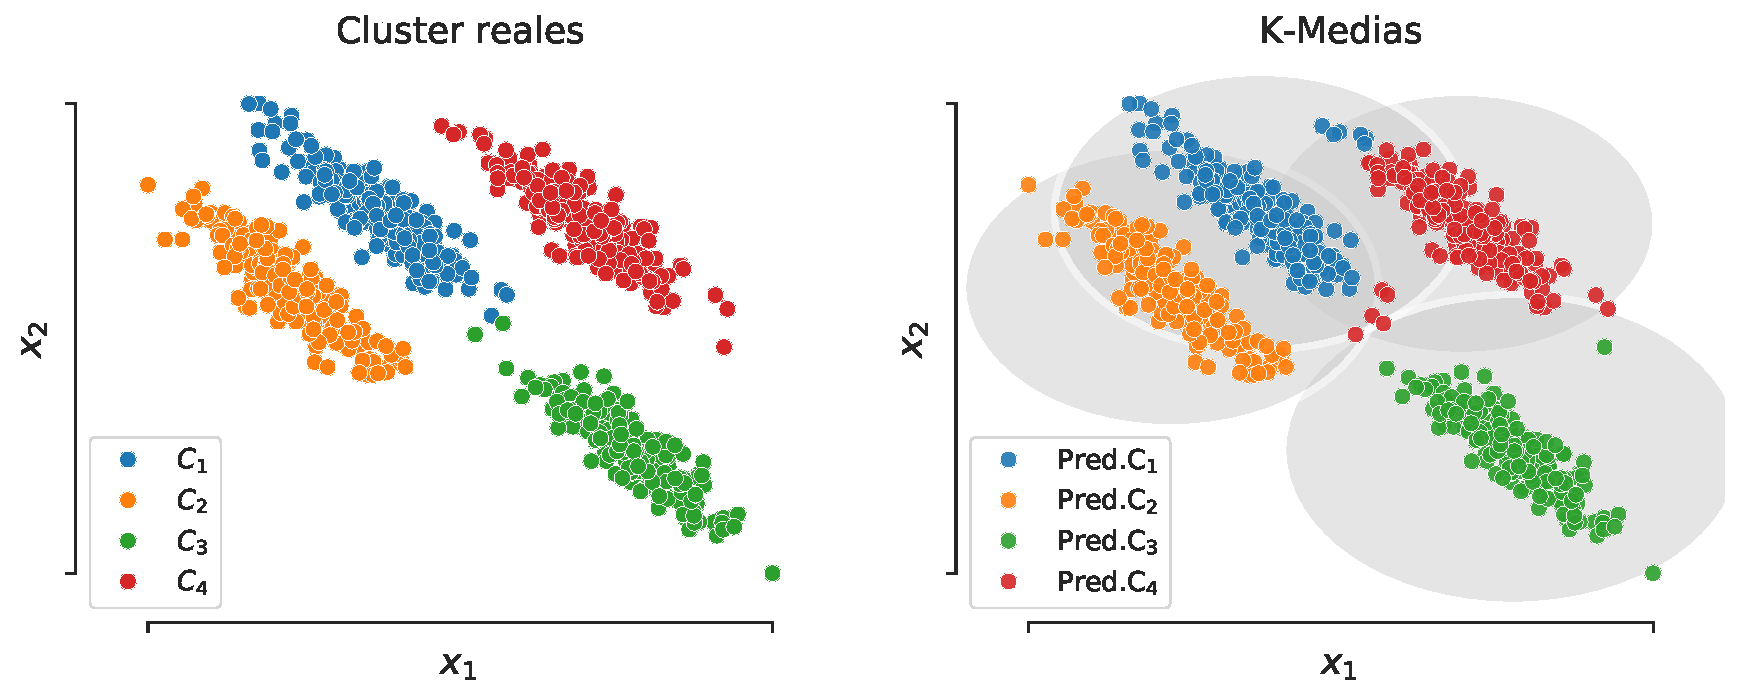
\includegraphics[width=0.7\textwidth]{img/cap6_k_medias}
  \caption{(Izquierda) Datos reales con sus etiquetas correctas. (Derecha) Clusters encontrados por k-means.}
  \label{fig:kmeans_1}
\end{figure}

Por otra parte, la asignación de cluster mediante el centroide más cecano provoca que cada par de centroides divida al espacio ambiente en dos semiespacios mediante el hiperplano simetral que pasa entre ambos puntos. Luego, dado que la intersección finita de semiespacios genera un poliedro, se tiene que la partición generada por kmeans forma un diagrama de Voronoi.

\begin{figure}[h]
  \centering
  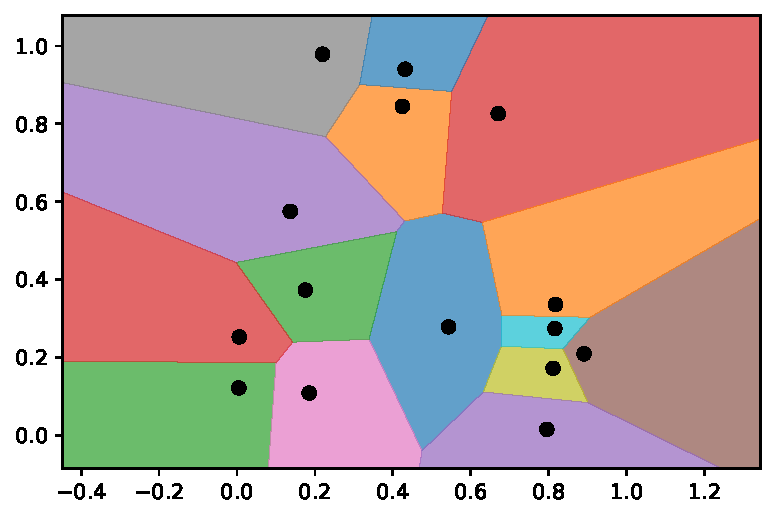
\includegraphics[width=0.6\textwidth]{img/cap6_voronoi}
  \caption{Partición de $\mathbb{R}^2$ inducida por los centroides.}
  \label{fig:kmeans_2}
\end{figure}


\subsubsection{Modelo de mezcla de gaussianas (GMM)}

La mezcla de gaussianas (GMM) es un caso general de $k$-means, en donde los clusters pueden tener una forma anisotrópica modelada por una Gaussiana con covarianza no necesariamente proporcional a la identidad. Además, si bien su solución puede ser muy similar a $k$-means los supuestos subyacentes al modelo CMM son diferentes y obedecen a un enfoque de modelo generativo. \\


Una distribución de mezcla de gaussianas consiste en una combinación convexa de distribuciones gaussianas
\begin{equation}
	p(\x) = \sum_{k=1}^K \pi_k \mathcal{N}(\x| \mu_k,\Sigma_k)
\end{equation}

Donde una muestra $x$ es generada mediante dos etapas: primero se elige un cluster al azar y luego, se genera una muestra aleatoria dentro del cluster. Nos referiremos a los parámetros de este modelo como 

\begin{itemize}
	\item $\pi_k:$ coeficiente de mezcla del cluster  $k$ (probabilidad de venir del cluster $k$).
	\item $\mu_k:$ media del cluster  $k$.
	\item $\Sigma_k:$ matriz de covarianza del cluster  $k$.
\end{itemize}

Para ver que la formulación anterior es la indicada para la generación de $\x$, se puede asignar una variable latente $\z(\x) = \z = [z_1,z_2,\ldots,z_K]^\top\in\{0,1\}^K$, que describa la asignación de $\x$ a cada cluster, es decir, $z_{k}=1$ si la observación $\x$ pertenece al cluster $k$, y $z_{k}=0$ si no. Bajo esta notación, podemos denotar la distribución marginal del cluster $k$ (es decir, de que una observación sea generada por la $k$-ésima componente) como 
\begin{equation}
 	p(z_k=1) = \pi_k \label{eq:GMM_marg1}
\end{equation} 

Además, para una muestra $\x$ proveniente del cluster $k$ se tiene que

\begin{equation}
	p(\x|z_k=1) = \cN(\x|\mu_k,\Sigma_k)
\end{equation}

Por lo tanto, usando probabilidades totales:

\begin{equation}
	p(\x)=\sum_{k=1}^N p(z_k=1) p(\x|z_k=1) = \sum_{k=1}^N \pi_k \cN(\x|\mu_k,\Sigma_k)
\end{equation}

Lo cual prueba que el modelo sugerido al comienzo es el indicado para una mezcla de gaussianas.\\

Recordemos que los parámetros del modelo de mezcla de gaussianas son los coeficientes de mezcla, las medias y varianzas de cada componente. Si disponemos de un conjunto de observaciones $\{\x_i\}_{i=1}^N$, entonces podemos encontrar dichos parámetros mediante máxima verosimilitud. Observe que la log-verosimilitud está dada por 

\begin{equation}
	\log p(\x_1,\ldots,\x_N) = \sum_{n=1}^N \log p(\x_n) = \sum_{n=1}^N \log \sum_{k=1}^K  \pi_k\cN(\x_n|\mu_k,\Sigma_k) \label{eq:GMM_like}	
\end{equation}
Hay una serie de complicaciones relacionados a la búsqueda de estos parámetros mediante la maximización de la ecuación \eqref{eq:GMM_like}. Primero, están las soluciones dadas por singularidades cuando una muestra es exactamente igual a una de las medias, en cuyo caso un término de la log-verosimilitud es proporcional a $1/\sigma_k$, con lo que la maximización de $\sigma_k$ resulta en una log-verosimilitud infinita. En segundo lugar tenemos las redundancias de soluciones: para cada máximo local (o solución en general) de la log-verosimilitd existen $k!$ soluciones equivalente con la misma verosimilitud dadas por las permutaciones de las etiquetas de los clusters. Finalmente, optimizar la log-verosimilitud de la mezcla de gaussianas es desafiante porque la sumatoria aparece \emph{dentro} del logaritmo, consecuentemente,  el logaritmo no actúa directamente en la gaussiana reduciendo el funcional de optimización a una solución en forma cerrada. Por esta razón, es necesario considerar métodos basados en gradiente.


\paragraph{Entrenamiento de una GGM}

Veamos las condiciones de primer orden sobre la log-verosimilitud para encontrar los parámetros. Denotando $\gamma(z_k(\x_i)) = p(z_k(\x_i)=1|\x_i)$, se tiene el siguiente resultado:

\begin{lemma} Para el modelo GGM, los parámetros óptimos son
	\begin{align}
    \mu_k & = \frac{1}{R_k}\sum_{i=1}^N \gamma(z_k(\x_i))\x_i\\
    \Sigma_k & = \frac{1}{R_k} \sum_{i=1}^N \gamma(z_k(\x_i))(\x_n - \mu_k)(\x_n - \mu_k)^\top\\
    \pi_k & = \frac{R_k}{R},
    \end{align}
    donde $R_k = \sum\limits_{i=n}^N \gamma(z_k(\x_i))$ y $R = \sum\limits_{k=1}^K R_k$.
\end{lemma}

Observe que esto no constituye una solución en forma cerrada para los parámetros, pues la posterior $\gamma(z_k(\x_i))$ depende de todos los parámetros, en efecto, gracias al teorema de Bayes:

\begin{align}
	p(z_k(\x)=1|\x) = \frac{p(\x|z_k(\x)=1)p(z_k(\x)=1)}{p(\x)} = \frac{\pi_k \cN(\x|\mu_k,\Sigma_k)}{\sum_{k=1}^K \pi_k \cN(\x|\mu_k,\Sigma_k)} 
\end{align} 


Sin embargo, podemos considerar un procedimiento iterativo en donde calculamos las posteriores $\gamma(z_k(\x_i))$ (llamado paso E), para luego calcular los parámetros óptimos de acuerdo a las ecuaciones anteriores (llamado paso M).\\

La Figura \ref{fig:gmm} muestra un ejemplo de clustering utilizando GMM. En este caso, se puede observar directamente como GMM es una generalización de $k$-means, en donde ahora los clusters tienen forma de gaussiana anisotrópica.

\begin{figure}[ht]
  \centering
  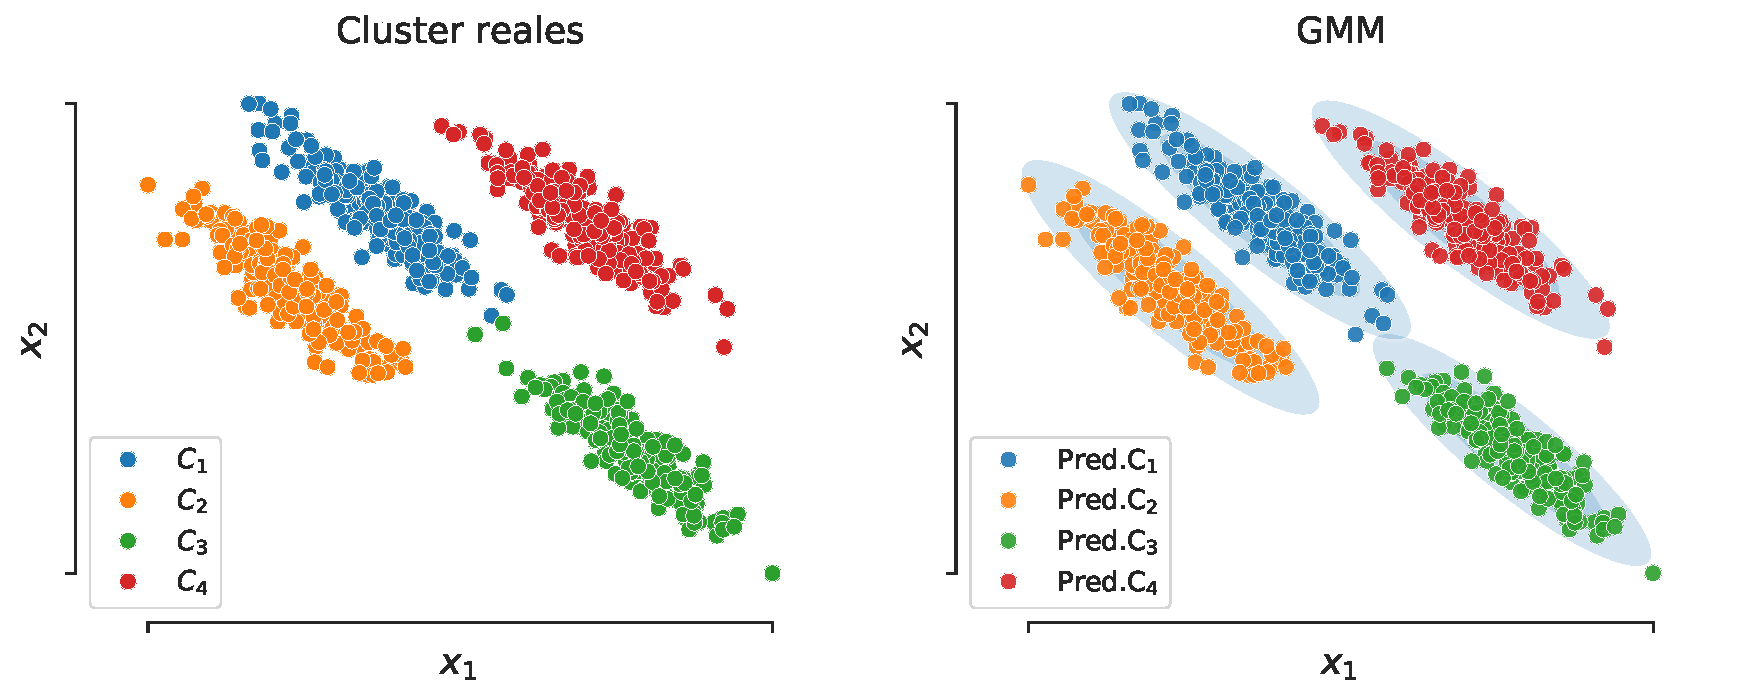
\includegraphics[width=0.8\textwidth]{img/cap6_gmm}
  \caption{(Izquierda) Datos reales con sus etiquetas correctas. (Derecha) Clusters encontrados por GMM.}
  \label{fig:gmm}
\end{figure}

 \begin{mdframed}[style=pendiente, frametitle={\center Expectation-maximization}]

En el caso general, tenemos \emph{observables} $\x$, variables latentes $\z$ y parámetros $\theta$, y un modelo descrito por una distribución marginal que puede ser expresada mediante 

\begin{equation}
	\log p(\x|\theta) = \log \int p(\x,\z|\theta)d\z
\end{equation}
donde el logaritmo de sumas es complicado de optimizar, incluso cuando la distribución conjunta $p(\x,\z|\theta)$ está en la familia exponencial.\\

Asumamos por un momento que tenemos valores para la variable latente $\z$, si este fuese el caso, podríamos buscar los parámetros mediante la optimización de la log-verosimilitud completa, $\log p(\x, \z |\theta)$, la cual como en GMM puede tener una forma más simple de optimizar debido a que no hay una suma dentro del logaritmo. \\

Sin embargo, en la prácticax no tenemos acceso al valor de las variables latentes $\z_n$ sino que únicamente podemos acceder a una estimación de estas mediante la distribución posterior $p(\z|\x,	\theta)$. Entonces, estrictamente hablado, la cantidad que nos gustaría maximizar $\log p(\x, \z |\theta)$ es aleatoria, por lo que podemos maximizar su esperanza con respecto a las observaciones (etapa de maximización). Luego, con los valores obtenidos para los parámetros podemos recalcular la distribución posterior $p(\z|\x,\theta)$ (etapa de esperanza) y seguir este proceso iterativamente. La motivación de este procedimiento, llamado \emph{expectation-maximization}, es que en primer lugar, con la cantidad $p(\z|\x,\theta)$ fija, el cálculo de los nuevos parámetros mediante máxima verosimilitud indiscutiblemente aumenta la verosimilitud, luego estos mejores parámetros dan consecuentemente una mejor estimación de la distribución posterior $p(\z|\x,\theta)$, con lo cual la actualización de los parámetros usando esta mejorada aproximación de la posterior debe ser incluso mejor.


\end{mdframed}


\subsubsection{Density-based spatial clustering of applications with noise (DBSCAN)}

Es un algoritmo de clustering propuesto por Martin Ester et al. el cual ha tenido mucha popularidad puesto que no requiere definir una cantidad inicial de clusters. Los hiper-parámetros de entrada del modelo son 2:

\begin{itemize}
    \item Mínimo número de punto: $minPts$.
    \item Radio o vecindad: $\epsilon$.
\end{itemize}

El algoritmo se basa en la idea de que dado 2 púntos $x_i$, $x_j$ dentro de un mismo cluster, se dice que \emph{$x_i$ es alcanzable por $x_j$}, si siempre se puede llegar de $x_i$ a $x_j$ avanzando de punto en punto, donde la distancia entre cada uno es a lo más $\epsilon$ y además un punto intermedio es un punto núcleo. Con estos el algoritmo define tres tipos de puntos:

\begin{itemize}
    \item \textbf{Puntos núcleo:} Son puntos $x_i$ tales que en una vecindad $\epsilon$ tienen almenos $minPts$ vecinos.
    \item \textbf{Puntos borde:} Constituyen el \textit{borde externo} de los cluster.
    \item \textbf{Outliers:} Puntos que no son alcanzables por ningún punto.
\end{itemize}

Notemos que con lo anterior, se desprende que todo cluster debe tener al menos un punto núcleo.
El algoritmo para encontrar los clusters es el siguiente:


\begin{algorithm}[H]
  \caption{Pseudo código de DBSCAN
    \label{DBSCAN}}
  \begin{algorithmic}[1]
    \Function{DBSCAN}{$D, eps, MinPts$}
      \State $C \gets 0$\;
      \For{{cada punto $P$ no visitado en $D$}}
      \State marcar $P$ como visitado
        \If{sizeOf(PuntosVecinos) $\le$ MinPts}
        \State marcar $P$ como RUIDO
        \Else
        \State C $\gets$ C+1
        \State expandirCluster(P,vecinos, C, eps, MinPts)
        \EndIf
      \EndFor
    \EndFunction
  \end{algorithmic}
\end{algorithm}


\begin{algorithm}[H]
  \caption{Función para expandir cluster.
    \label{alg:expandirCluster}}
  \begin{algorithmic}[1]
  \Function{expandirCluster}{P, vecinosPts, C, eps, MinPts}
  \State agregar P al cluster C
  \For{cada punto P' en vecinosPts}
  \If{P' no fue visitado}
         \State marcar P' como visitado\;
         \State vecinosPts' $\gets$ regionDeConsulta(P', eps)\;
         \If{sizeof(vecinosPts') $\geq$ MinPts}
            \State vecinosPts $\gets$ vecinosPts $\cup$ vecinosPts'
        \EndIf
    \EndIf
    \If{P' no tiene cluster asignado}
         \State P' se le asigna el cluster C
    \EndIf
    \EndFor
    \EndFunction
  \end{algorithmic}
\end{algorithm}


\begin{algorithm}[H]
  \caption{Retorna los puntos de la vecindad de búsqueda para un punto.
    \label{alg:regionDeConsulta}}
  \begin{algorithmic}[1]
    \Function{regionDeConsulta}{$P, eps$}
    
    \Return Todos los puntos junto a P' que están a eps de distancia (incluyendo P)
    \EndFunction
  \end{algorithmic}
\end{algorithm}

La figura \ref{fig:dbscan} muestra un ejemplo de clustering utilizando DBSCAN. A la derecha se muestran en negro los puntos que son clasificados como ruido o \emph{outliers} por el algoritmo. Por otro lado, los puntos núcleos son graficados como un punto grande, mientras que los puntos borde se grafican con un marcador pequeño.

\begin{figure}[H]
  \centering
  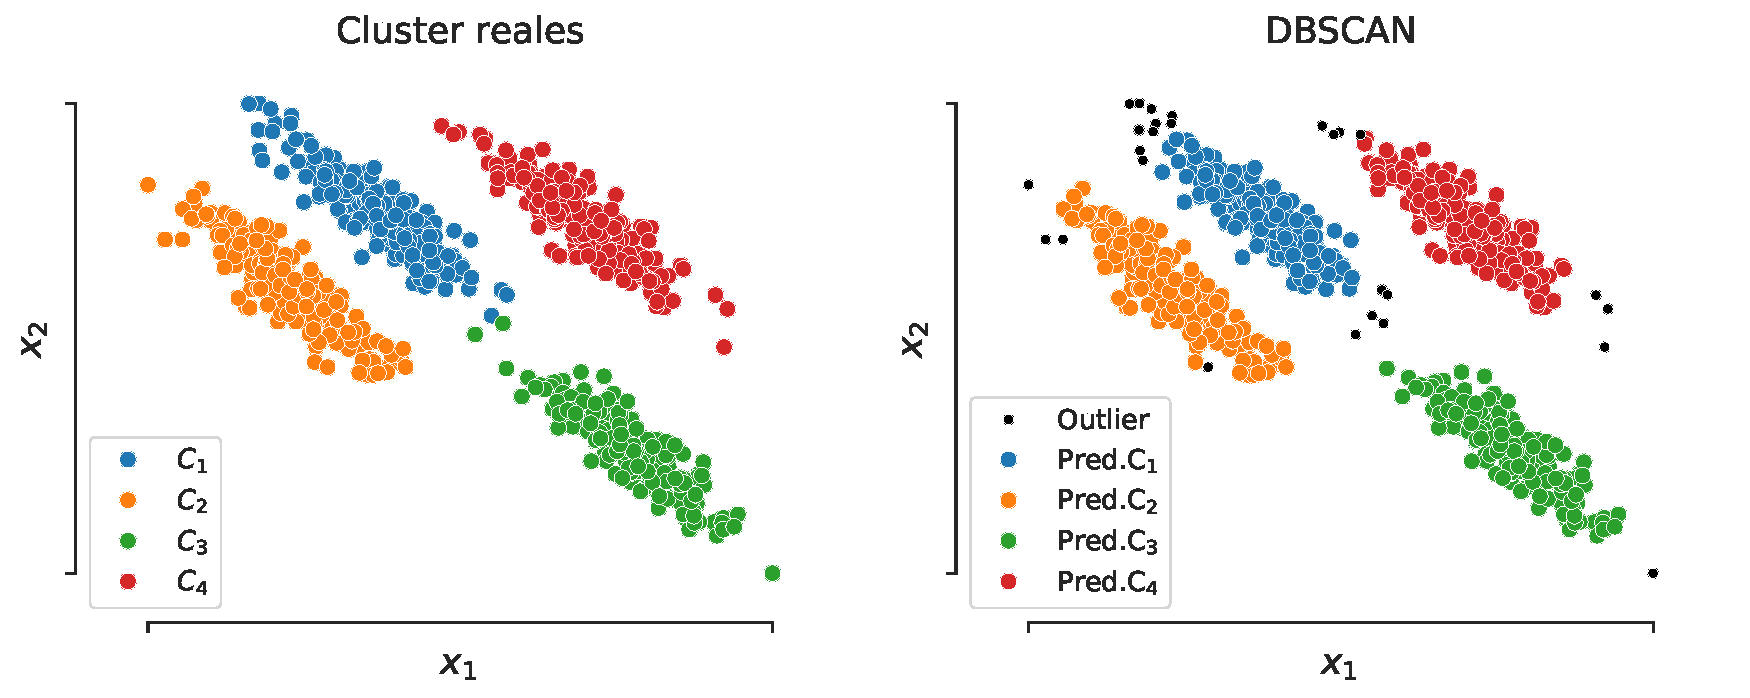
\includegraphics[width=0.8\textwidth]{img/cap6_dbscan}
  \caption{Datos reales con sus etiquetas correctas (izquierda) y clusters encontrados por DBSCAN (derecha).}
  \label{fig:dbscan}
\end{figure}

\subsubsection{Aprendizaje Semi-Supervisado}

Como el lector debe haber notado a este punto, todos los modelos anteriores son útiles siempre y cuando las características que se den como input al modelo permitan resumir y estudiar los datos de buena manera. Sin embargo, esta tarea no es nada fácil: Muchas veces los \textit{features} que permiten llegar a un modelo son desconocidos o muy difíciles de encontrar. \\

Una propuesta para solucionar la problemática anterior es usar métodos de aprendizaje no supervisado para obtener \textit{features}, y usarlos como input de un modelo supervisado. En otras palabras, se ocupa un modelo no supervisado para pre-procesar los datos. Es así que surge así el término de aprendizaje semi-supervisado. \\

Existen casos en la bibliografía donde modelos supervisados generalizan mejor cuando hay preprocesamiento mediante métodos no supervisados. \\

En particular, es muy común ocupar K-Means como preprocesamiento. Este proceso se sintetiza en los siguientes pasos: 

\begin{enumerate}
    \item Encontrar un número de clusters óptimos para el conjunto de entrenamiento.
    \item Calcular la distancia a cada cluster para todo el conjunto de entrenamiento. 
    \item Usar las distancias a cada clusters como input a un modelo supervisado (por ejemplo, una regesión logística). 
\end{enumerate}

\subsubsection{Otros Algoritmos de Clustering}

Los algoritmos de clustering que fueron presentados son sólo los más comunes. Sin embargo, existen otros algoritmos que pueden ser útiles en la práctica. En esta sección mencionaremos brevemente algunos de ellos. 

\begin{itemize}
    \item \textbf{BIRCH}: 
    
    El algoritmo BIRCH  (\textit{Balanced Iterative Reducing and Clustering using Herarchies}) fue diseñado específicamente para datsets muy grandes. Es más rápido que K-Means con batches, y con resultados parecidos con una cantidad de features baja ($< 20$). Su innovación es en el uso de memoria para asignar un dato a un cluster en particular.
    \item \textbf{Spectral Clustering}:
    Este algoritmo crea una matriz de similitud entre los datos, y reduce su dimensionalidad. Luego de esto, se ocupa otro algoritmo de clustering (por ejemplo, K-Means) en este espacio de dimensión baja. \\
    
    Este algoritmo puede encontrar relaciones muy complejas en los datos, sin embargo no escala bien a grandes cantidades de datos, ni tampoco se comporta bien cuando los clusters están desbalanceados. 
\end{itemize}
